\documentclass[output=paper]{langsci/langscibook} 
\ChapterDOI{10.5281/zenodo.1441343}
\author{Olga Kellert\affiliation{Georg-August-Universität Göttingen}\and Daniele Panizza\affiliation{Georg-August-Universität Göttingen}\lastand Caterina Petrone\affiliation{Laboratoire Parole et Langage, Aix-Marseille Université}}
\title{On the role of prosody in disambiguating wh-exclamatives and wh-interrogatives in Cosenza Italian}
\shorttitlerunninghead{wh-exclamatives and wh-interrogatives in Cosenza Italian}
% \chapterDOI{} %will be filled in at production \textit{wh-}
 
\abstract{This work investigates the role of prosody in the perception of \textit{wh-}exclamatives and (information-seeking) \textit{wh-}interrogatives in Cosenza Italian, a Southern Italian variety spoken in Calabria. Following recent research on prosody, we use a two-alternative forced-choice identification task in combination with reaction time measurements, as reaction times have been used as a better substitute of discrimination scores to investigate categorical perception of prosodic contrasts. Here, this methodology is preferred to more difficult offline tasks (e.g. the gating paradigm) to test to what extent phonetic/phonological cues distributed over the utterance might guide listeners' responses during sentence type identification. Our results show that listeners identify the two sentence types after the end of the utterance in most of the trials, not before it. This suggests that prosodic cues that occur before the end of the utterance (e.g. in the prenuclear section of the intonational contour) are not strong enough by themselves to guide the pragmatic interpretation of the utterances. Furthermore, our study shows that exclamatives are processed faster than interrogatives, but this effect disappears when segmental duration is taken into account.}
\maketitle

\begin{document}
\label{chap:kel}\label{ch:5}
 

  
% Keywords: Reaction Times, wh-exclamatives, wh-interrogatives, prosody, perception, Cosenza Italian
 

\section{Introduction}

While in languages such as English, \textit{wh-}exclamatives and information-seeking \textit{wh-}interrogatives (hereafter “\textit{wh-}interrogatives”) are syntactically differentiated (e.g. \textit{How many books you have read!} vs. \textit{How many books have you read?}), in Italian the two sentence types are syntactically the same: 



\ea\label{ex:kel:1}
Italian \textit{wh-}exclamatives

\gll Quanti    romanzi  ha  scritto   la  tua  amica! \\
     How~many  novels   has written   the your friend\\
\glt `How many novels your friend wrote!'
\z


\ea\label{ex:kel:2}
 Italian \textit{wh-}interrogatives

\gll Quanti     romanzi  ha  scritto   la   tua amica?    \\
     How~many   novels   has written   the your friend\\
\glt `How many novels did your friend write?'
\z


Studies on different languages have already shown that when syntactic structure is ambiguous, listeners mainly rely on prosodic information to identify exclamatives and interrogatives (cf. \citealt{Batliner1988,Eady1986,Sorianello2011exclamative,Sorianello2012,Gyuris2013}). 

However, it is still unclear to what extent temporally distributed phonological/phonetic properties are exploited by listeners for sentence-type identification. Consider the Italian examples in (\ref{ex:kel:1}) and (\ref{ex:kel:2}). The prosodic cues that determine the exclamative/interrogative meaning of these sentences could be contained in the \textit{wh-}phrase (`how many novels’), in the verb phrase (`has written’), or in the final subject phrase (`your friend’). In the variety spoken in Cosenza (Southern Italy), \textit{wh-}exclamatives and \textit{wh-}interrogatives contain different prosodic cues in both the prenuclear region (i.e. at the beginning of the intonation contour) and in the nuclear region (i.e., at the end of the intonation contour). \textit{wh-}exclamatives exhibit a \%H at the left edge of the intonational phrase, which is absent in \textit{wh-}interrogatives (where a prenuclear accent H* is produced on the \textit{wh-}constituent; see \citealt{Sorianello2012} and \sectref{sec:kel:2} for details). Furthermore, the two sentence types are differentiated in the nuclear-accent choice associated with the verb phrase (L* in \textit{wh-}exclamatives vs. L+H* in \textit{wh-}interrogatives; ibid.).

Our study, focusing on Cosenza Italian, addresses two main questions. First, we ask whether listeners rely on the nuclear information alone or whether the prenuclear region also contributes to the perception of sentence type. Given that \%H might differ from the prenuclear H* in many F0 dimensions (such as tonal alignment and pitch excursion), we hypothesize that listeners should be able to discriminate the two sentence types from the beginning.

This question is linked to the issue in intonation research of how intonational meaning is created. The Autosegmental-Metrical (AM) framework assumes that the nuclear pitch accent is merely the last accent within a specific major prosodic phrase (cf. \citealt{Ladd2008} for a review). The overall meaning of a tune results from the independent contributions of its freely combinable, morpheme-like sub-parts, which include pitch accents and edge tones (\citealt{Pierrehumbert1990}). Despite this compositional-based approach to tune meaning, work within the AM theory often regards the nucleus – more or less implicitly – as the semantic “heart” of the tune. Hence, the current study searches for the meaning contribution of the prenuclear region and its potential interaction with the nuclear tune.

Furthermore, we ask whether the processing of the intonational contour is similar between the two sentence types or whether some cues are more salient in one sentence type than in the other. The \%H is a marked pattern in Italian, since its use is restricted to a few contexts (including the \textit{wh-}exclamatives). It also exhibits enhanced pitch excursion, which renders it perceptually salient (\citealt{Sorianello2012}). Hence, we hypothesize that the intonation of \textit{wh-}exclamatives should be processed and identified much faster than the intonation of \textit{wh-}interrogatives.

Concerning methodology, we employ an experimental design that involves an identification task with measurement of reaction times. Identification tasks have been already used in combination with reaction times (RTs) in prosody research, especially within the categorical perception paradigm (\citealt{Chen2003,Fale2006,Niebuhr2007,Feldhausen2011}, among others). Reaction times are believed to reflect task difficulty (\citealt{Massaro1987}) and they have been used as a substitute for discrimination scores to test whether the perception of prosodic contrasts is categorical or gradient (\citealt{Chen2003,Niebuhr2007}). This methodology has been applied to contrasts at the level of pitch accents (\citealt{Chen2003,Niebuhr2007,Feldhausen2011}), prosodic boundaries (\citealt{Schneider2011,Petrone2017}), and global phonetic cues (such as pitch range; see \citealt{Borras-Comes2010}). The studies in question are all based on manipulated stimuli. Given a continuum of manipulated stimuli, it is generally supposed that, in the case of categorical boundary perception, reaction times should be long at the location corresponding to the category boundary and short in other parts of the continuum. In contrast, a gradual increase in reaction time with proximity to the boundary might reflect a gradual increase of the ambiguity of the stimuli, pointing to a more gradient boundary perception. In the current study, we will measure identification scores and reaction times in response to natural (not manipulated) stimuli as a first step in the investigation of an understudied prosodic contrast, i.e. the contrasts between \textit{wh-}exclamatives and \textit{wh-}interrogatives.

The structure of the paper is as follows: After a short review of the literature on \textit{wh-}exclamatives and \textit{wh-}interrogatives (\sectref{sec:kel:2}), the goals of the study will be stated (\sectref{sec:kel:3}) and a description of the experiment will be given (\sectref{sec:kel:4} and \sectref{sec:kel:5}). The findings will be discussed in \sectref{sec:kel:6}. Finally, the benefits and the challenges of the chosen methodology will be discussed in \sectref{sec:kel:7}.


\section{Previous investigations of the prosody of \textit{wh-}exclamatives and \textit{wh-}interrogatives}
\label{sec:kel:2}

Prosodic characteristics of \textit{wh-}interrogatives have been extensively studied in many languages (e.g. \citealt{Zeng.2004,Hedberg2010,Vanrell2013whquestions}). Concerning Italian, one of the most typical intonational characteristics of \textit{wh-}in\-ter\-ro\-ga\-tives is the presence of utterance-final F0 fall (\citealt{Chapallaz1964,Avesani1995,Sorianello2011exclamative}). However, the intonational pattern of \textit{wh-}interrogatives can vary in many respects depending on their pragmatic function (e.g. rhetorical vs. information-seeking; see \citealt{Hedberg2010}) and on the regional variety (see \citealt{Avesani1995,Sorianello2011exclamative,GiliFivelaETAL2015intonationalvariation}, among others). In particular, in Cosenza Italian, the nuclear accent of information-seeking \textit{wh-}interrogatives is associated with a rising accent L+H* followed by a low boundary tone L\% (see \citealt{Sorianello2011exclamative,Sorianello2011CosenzaPowerPoint}).

Differently from \textit{wh-}interrogatives, research on prosody of \textit{wh-}exclamatives is cross-linguistically scarce (see \citealt{Batliner1988,Sorianello2011exclamative,Gyuris2013}). Studies so far have rather focused on the syntactic and semantic differences between \textit{wh-}exclamatives and \textit{wh-}interrogatives (see \citealt{Portner2003,Castroviejo2006}, among others). \textit{wh-}exclamatives and \textit{wh-}interrogatives would mainly differ with respect to factivity, i.e., exclamatives imply a true proposition and interrogatives do not. \citet{Portner2003} deduce the factivity of \textit{wh-}exclamatives from two considerations. First, exclamatives (including \textit{wh-}exclamatives) can be embedded under factive predicates only \citep[46]{Portner2003}:

\ea\label{ex:kel:3}
 Mary knows/*thinks/*wonders how very cute Mario is.   \\
\z

Furthermore, \textit{wh-}exclamatives can never be used as questions and never induce a response from the interlocutor:

\protectedex{
\ea\label{ex:kel:4}
\ea
A: How tall is Mary? B: 1.80. \\
\ex
A: How tall Mary is! B: \#1.80. \\
\z
\z
}

Some studies have shown that prosodic information alone might be used to distinguish (\textit{wh-} and non-wh) exclamatives from other sentence types. Exclamatives have been claimed to be cross-linguistically characterized by an initial extra-high pitch followed by a falling intonation contour (see \citealt{OConnor.1961} for English; \citealt{Delattre1966} for French; \citealt{DEugenio1976} for Italian; \citealt{Batliner1988} for German). However, in some languages, such as Hungarian, exclamatives are instead characterized by an initial low pitch (a low boundary tone; see \citealt{Gyuris2013}). Concerning the nuclear region, \citet{Gyuris2013} found that Hungarian listeners classified acoustic stimuli as exclamatives and not as interrogatives if they included nuclear pitch accents with rising F0 pattern; delayed peaks; and a combination of low initial boundary tones and rising accents.

Concerning Cosenza Italian, \citet{Sorianello2011exclamative} provides a phonological analysis of both \textit{wh-}exclamatives and \textit{wh-}interrogatives (see also \citet[182]{GiliFivelaETAL2015intonationalvariation} on \textit{wh-}interrogatives in Cosenza Italian and other Italian varieties). The two sentence types are characterized by the same ending, i.e., a L-L\% tonal sequence (see \figref{fig:kel:1} and \figref{fig:kel:2}).  However, they are differentiated phonologically in the regions preceding the utterance’s final fall, i.e., both at the left edge of the intonational phrase (IP) and within the nuclear region. First, the initial part of \textit{wh-}exclamatives is marked by a high boundary tone at the left edge of the IP (represented by \%H in \figref{fig:kel:1}), which is not present in \textit{wh-}interrogatives (for \%H in non-\textit{wh-}exclamatives, see \citealt{Sorianello2012,Avesani1995,Grice2005}). \textit{Wh-}interrogatives are characterized by a prenuclear accent L+ H* on the \textit{wh-}constituent (see \figref{fig:kel:2}). Moreover, the nuclear accent is specified differently, i.e., a low accent L* characterizes \textit{wh-}exclamatives and a rising accent L+H* appears in \textit{wh-}interrogatives. Along with the intonational cues, \textit{wh-}exclamatives are also characterized by an extra lengthening of the duration of the nuclear-stressed syllable \citep{Sorianello2011exclamative}.

While there are still no perception studies on \textit{wh-}exclamatives in Cosenza Italian, there are studies of non-\textit{wh-}exclamatives in other Southern varieties of Italian that suggest that the prenuclear region can contribute to their identification. In an experiment on Bari Italian, \citet{Sorianello2012} used natural minimal pairs of non-\textit{wh-}exclamatives and assertions, cutting the sentences at different temporal locations. This procedure is reminiscent of the gating procedure used in word-recognition research to investigate the uptake of acoustic-phonetic cues to segmental structure (\citealt{Grosjean1980,Lahiri1991}, inter alia; see \citealt{Petrone.2011} for an example of this technique applied to intonational contrasts). \citet{Sorianello2012} found that listeners could identify non-\textit{wh-}exclamatives when only the initial part of the contour was available. By contrast, the prenuclear contour did not seem to provide robust cues for identifying assertions. Thus, the prenuclear cues are not equivalent across sentence types. 

\begin{figure}

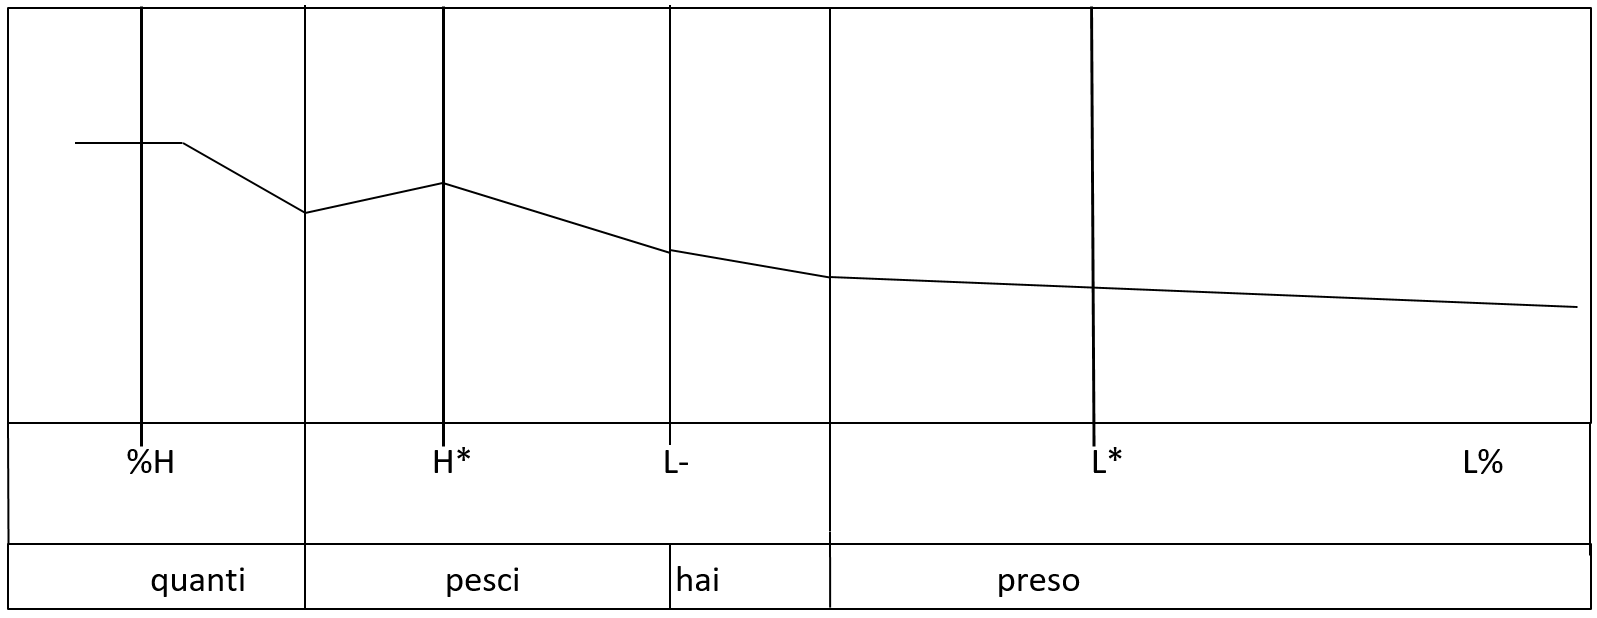
\includegraphics[width=0.99\textwidth]{figures/KEL-img1.PNG}
\caption{Our schematized version after \citeauthor{Sorianello2011exclamative}´s (\citeyear[316]{Sorianello2011exclamative}) representation of \textit{Quanti pesci hai preso!} ‘How many fishes you took!’}
\label{fig:kel:1}
\end{figure}


\begin{figure}
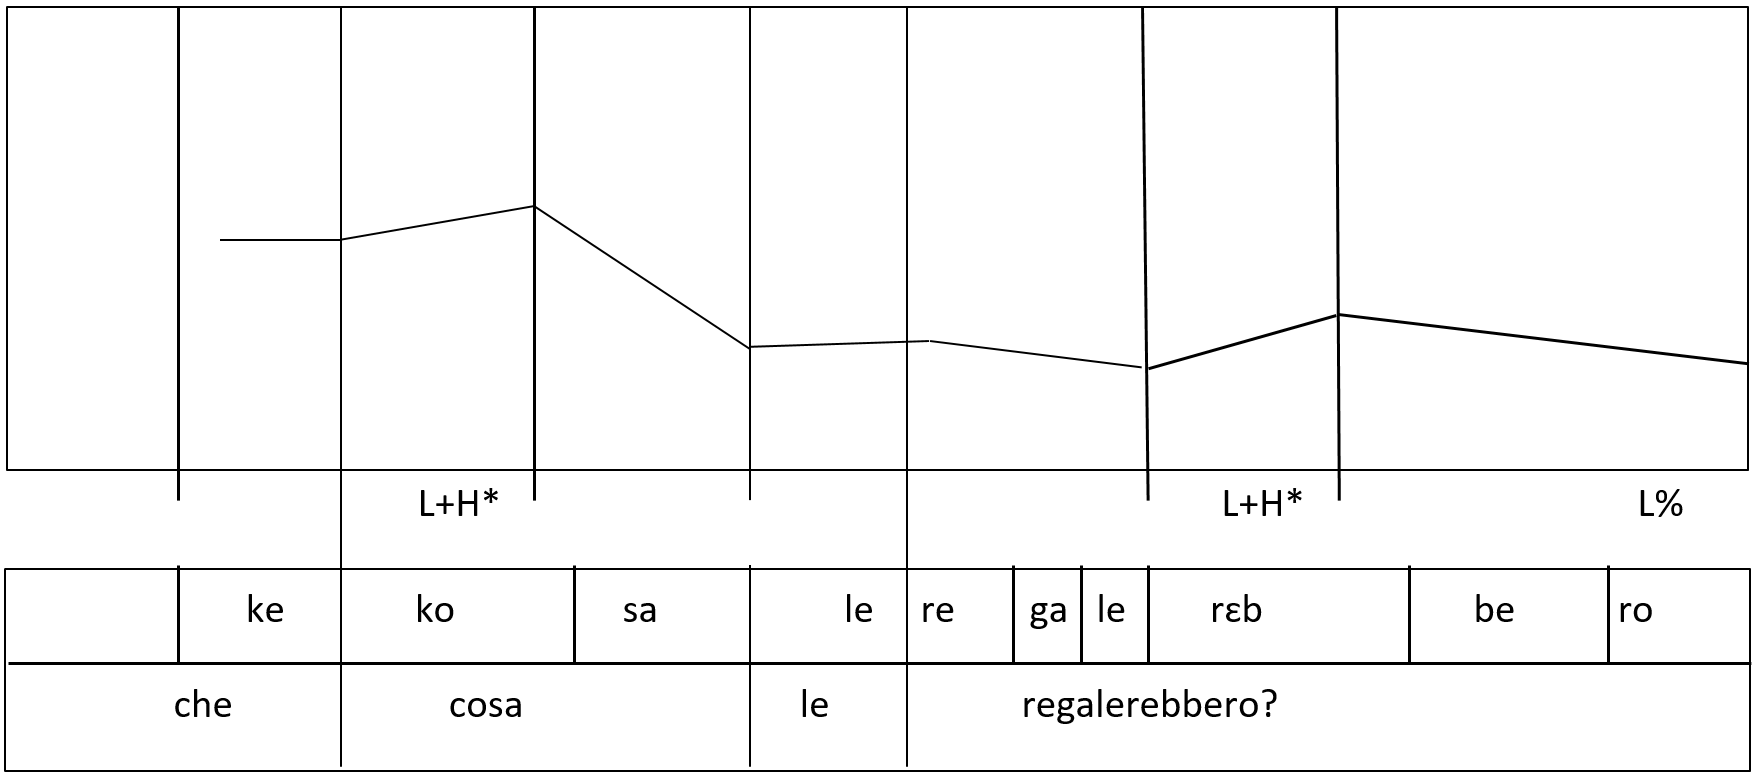
\includegraphics[width=0.99\textwidth]{figures/KEL-img2.PNG}
\caption{Our schematized version after the representation of Information-seeking \textit{wh-}interrogative: \textit{Che cosa le regalerebbero?} ‘What would they give her as a present?’ in \citep[182]{GiliFivelaETAL2015intonationalvariation}}
\label{fig:kel:2}
\end{figure}


\section{Goals of the study}
\label{sec:kel:3}

The main goal of this study is to determine if prosodic cues play an important role in the disambiguation of \textit{wh-}exclamatives and \textit{wh-}interrogatives in Cosenza Italian. Given the phonetic/phonological contrasts between the two sentence types that were described in \sectref{sec:kel:2}, listeners should be capable of distinguishing \textit{wh-}interrogatives from \textit{wh-}exclamatives on the basis of prosody (Hypothesis 1).

In particular, we seek to determine to what extent phonetic/phonological cues distributed over the utterance might guide listeners' responses. Given that the contrast between \textit{wh-}exclamatives and \textit{wh-}interrogatives should be noticeable already in the prenuclear region \citep{Sorianello2011exclamative}, we expect listeners to identify both sentence types before they hear the end of the sentence, with differences in the nuclear accent further helping perceptual disambiguation (Hypothesis 2).

Finally, we investigate the existence of potential differences in the processing of the two sentence types. Our hypothesis is that these processing differences do exist, since \textit{wh-}exclamatives but not \textit{wh-}interrogatives show a high boundary tone right at the beginning of the utterance, which is marked in Italian (i.e. \%H at the left edge of the intonational phrase) (see \citealt{Sorianello2011exclamative}). We thus assume that the intonation of \textit{wh-}exclamatives should be processed and identified much faster than the intonation of \textit{wh-}interrogatives (Hypothesis 3).

In order to test the three hypotheses, we conducted a two-alternative forced-choice identification task combined with measurement of reaction times. Our expectation was that identification scores should depend on differences in prosody between the two sentence types. Specifically, cues in the prenuclear region should enable disambiguation between \textit{wh-}exclamatives and \textit{wh-}interrogatives, even\linebreak though robust identification is only expected after the listener hears the entire utterance. Moreover, longer reaction times are expected to indicate higher uncertainty with respect to sentence-type identification, which should then be associated with lower identification scores in the identification task.



\section{Experiment}
\label{sec:kel:4}

\subsection{Experimental stimuli} 
\label{sec:kel:4.1}

We constructed 20 pairs of morpho-syntactically and lexically identical \textit{wh-}ex\-cla\-ma\-tives and \textit{wh-}in\-ter\-ro\-ga\-tives (like those in \ref{ex:kel:1} and \ref{ex:kel:2}). Each target sentence had a syntactic structure as in (\ref{ex:kel:5}): a complex \textit{wh-}constituent (i.e., \textit{quanti} ‘how many’ + noun); a verb phrase consisting of an auxiliary and a past participle; and a nominal constituent including a grammatical subject. (The definite article preceding the subject constituent was omitted in the case of immediate family members, as typical in Italian.)

\protectedex{
\ea\label{ex:kel:5}
Stimuli

\gll [Quanti romanzi] [ha  scritto]   [la   tua    amica]\\
     how~many novels     has written       the your friend\\
\glt ‘How many novels your friend wrote!’ or \\
\glt ‘How many novels did your friend write?’ 
\z
}

In order to elicit different intonation patterns in \textit{wh-}exclamatives and \textit{wh-}interrogatives, we embedded the stimuli in pragmatic contexts that only matched one or the other sentence type, such as in (\ref{ex:kel:6}) and (\ref{ex:kel:7}):


\ea\label{ex:kel:6}
\textit{wh-}exclamative context: Your mother tells you that her friend spent 10 years of her life writing novels and shows you a list of her books. You exclaim:

\gll Quanti  romanzi   ha  scritto   la   tua    amica! \\
     how~many   novels has written   the  your friend\\
\glt ‘How many novels your friend wrote!’
\z


\ea\label{ex:kel:7}
\textit{wh-}interrogative context: Your mother tells you that her friend spent 10 years of her life writing novels. You ask your mom:

\gll Quanti   romanzi  ha  scritto   la   tua    amica?    \\
     how~many novels   has written   the your friend\\
\glt ‘How many novels did your friend write?’
\z


The sentences were produced by a 38-year-old female speaker from Cosenza. The speaker silently read the contexts and then uttered the sentences aloud. She was instructed to produce the sentences in a natural way.\footnote{The discourse context was only presented in the production of the stimuli, to elicit a specific intonation contour, not in the identification task, since it would bias the responses of the listeners.} No instructions were given as to what specific prosodic pattern to use in sentence production. The 40 target sentences were presented randomly and interspersed with 20 fillers: non-\textit{wh-}interrogatives and non-\textit{wh-}exclamatives such as ‘Do you like coffee?’ ‘Open the door!’ and ‘I came late today’ (a yes-no interrogative, an imperative, and a declarative, respectively). A complete list of the experimental target sentences and the fillers is given in the Appendix.

For the perception experiment, \textit{wh-}exclamatives and \textit{wh-}interrogatives constituted our auditory target stimuli. For each sentence, we identified four critical points or “marks” (M) at sequential temporal locations: M1 = the beginning of the utterance; M2 = the end of the \textit{wh-}constituent; M3 = the end of the verb phrase; and M4 = the end of the subject constituent, which is also the end of the utterance. In example \REF{ex:kel:8} below, M1 is represented by an opening bracket and M2–M4 by closing brackets.


\ea\label{ex:kel:8}
\gll [=M1 Quanti romanzi]=M2 ha scritto]=M3  la   tua    amica]=M4 \\
 ~ how~many novels     has written       the your friend\\
\glt ‘How many novels your friend wrote!’ or \\
\glt ‘How many novels did your friend write!’ 
\z


The four marks divided the experimental sentences into three regions. The initial region, between M1 and M2, consisted of the \textit{wh-}constituent (e.g. \textit{Quanti romanzi}); the middle region, between M2 and M3, consisted of the verb phrase (e.g. \textit{ha scritto}); and the final region, from M3 to M4, consisted of the subject phrase at the end of the utterance (e.g. \textit{la tua amica}).


  
\subsection{Tasks and procedure}
\label{sec:kel:4.2}

Since it has been shown that there are durational differences between the two sentence types (cf. \citealt{Sorianello2011exclamative}), something that was also clear from an initial analysis of our data, we measured the duration of each region. Statistical analysis of the duration showed that the initial region was significantly longer in the exclamative condition than in the interrogative one (on average, excl. = 616 ms vs. inter. = 546 ms, p < .01). The verb phrase was not significantly different between the two conditions (excl. = 592 ms vs. inter. = 604 ms, p = .40). The final subject phrase was longer in the exclamative condition (excl. = 933 ms vs. inter. = 751 ms, p < .001). Given that the duration of different regions seemed to play a crucial role in identification, this parameter was included as a variable in the statistical models (see \sectref{sec:kel:6}).  

Eighteen monolingual Italian native speakers (aged between 19 and 34 years) participated in the perception study and were reimbursed for their time. The group was composed of 10 women and 8 men. They were all from the Cosenza area and were either university students or employees at the \textit{Università della Calabria}, in Cosenza. They reported no hearing problems.

Participants were asked to report which sentence type (\textit{wh-}exclamative vs. \textit{wh-}interrogative) better matched their auditory impression of the sentence. They were instructed to carefully listen to the stimuli and to press a button as soon as they were certain of the sentence type. 

This instruction was given in order to elicit as many early responses as possible, to enable us to check whether listeners could identify the sentence type before the end of the utterance (e.g. just from hearing the initial region, or the initial and middle regions). Before the experiment, listeners had a short practice session, with four practice sentences to identify. They did not receive any feedback on their answers. 

The identification task lasted about 10 minutes for each listener. Their responses and reaction times (measured from the offset of the stimulus) were re\-cor\-ded. Stimulus presentation and response collection were performed by an open-source toolkit based on the Python module Pygame (cf. Peirce 2007 for an overview of PsychoPy, a toolkit based on the same system).\footnote{The module can be downloaded for free together with the data from this experiment (danielepanizza.org/pages/programming).}

Each trial began with a written question to the participant/listener asking if they were ready to start. A beep was used to signal that an utterance was about to start, in order to draw the participant’s attention to the stimulus. The session began with the presentation of the auditory stimulus. For each listener, the identification task was broken into two blocks of 30 sentences, with some stimuli repeated in the second block. The goal of this manipulation was to check whether repetition of the same sentences influenced reaction times (\citealt{Bentin1994}). Block 1 contained 10 \textit{wh-}exclamative sentences and 10 \textit{wh-}interrogative sentences that were not lexically identical (“non-minimal-pair condition”). Stimuli were presented in random order and interspersed with 10 fillers (non-\textit{wh-}exclamatives and non-\textit{wh-}interrogatives). Block 2 also contained 10 \textit{wh-}excla\-ma\-tives, 10 \textit{wh-}interrogatives, and 10 fillers. This time, 5 of the 10 \textit{wh-}exclamatives were lexically identical to 5 of the 10 \textit{wh-}interrogatives presented in the first block, and likewise 5 of Block 2’s \textit{wh-}interrogatives were lexically identical to 5 of Block 1’s \textit{wh-}exclamatives. In other words, each participant heard 10 sentences under both the exclamative and the interrogative condition (“minimal-pair condition”, e.g. ‘How many novels has your friend written?’ vs. ‘How many novels your friend has written!’). In total, then, each participant heard 60 sentences: 20 \textit{wh-}exclamatives, 20 \textit{wh-}interrogatives, and 20 fillers. The stimuli were divided into four counter-balanced lists, to which listeners were randomly assigned. Listeners were tested one at a time in a quiet room. 


\section{Statistical analysis and results}
\label{sec:kel:5}

Before going into detail regarding the statistical analysis, we summarize our results with respect to the hypotheses we formulated in section 3. Our results show that:

Hypothesis 1 is confirmed. Listeners are very accurate in distinguishing \textit{wh-}exclamatives from \textit{wh-}interrogatives solely on the basis of prosody. 

Hypothesis 2 is partially confirmed. Listeners can distinguish between these two sentence types before they hear the end of the sentence, but this pattern is very rare in our data; much more often, listeners identified the sentence type after the end of the sentence. 

Hypothesis 3 is partially confirmed. Listeners are faster at identifying \textit{wh-}exclamatives than \textit{wh-}interrogatives. However, this effect is the result of durational differences between the two sentence types, so that the processing advantage for \textit{wh-}exclamatives disappears when the segmental duration is taken into account.

   
\subsection{Identification task}
\label{sec:kel:5.1}
Accuracy of sentence-type identification was very high in both experimental conditions. Listeners correctly identified exclamatives in 93.4\% of the trials and interrogatives in 93.7\% of the trials. Although listeners were instructed to make their choice as soon as possible, the great majority of responses were provided after the end of the utterance (“late” responses: 90.7\% for \textit{wh-}exclamatives and 92.0\% for \textit{wh-}interrogatives). As shown in \tabref{tab:kel:1}, in only 31 trials in the \textit{wh-}exclamative condition and 27 trials in the \textit{wh-}interrogative condition did listeners provide “early” responses (i.e., before the end of the utterance). Early responses were mostly correct, suggesting that some listeners are indeed able to discriminate the prosody of the two sentence types before the end of the utterance. For \textit{wh-}exclamatives, the error rate for early responses was 19\% compared to 5\% for late responses, while for \textit{wh-}interrogatives, the error rates were 4\% for early responses and 6\% for late responses. These results suggest that listeners were more prone to error when providing an early answer in response to \textit{wh-}exclamatives than to \textit{wh-}interrogatives. However, the difference between correct and incorrect early responses could not be assessed statistically because of the low number of observations. 

We ran a generalized linear mixed model (GLMM) in order to analyze the accuracy of late responses. We adopted \textit{sentence type} (interrogative vs. exclamative) and \textit{block} (Block 1 vs. Block 2) as fixed factors and \textit{item} (i.e. the lexical material) and \textit{participant} as random factors, with maximal random-effect structure (cf. \citealt{Barr2013}), that is, with the greatest possible number of free slopes and intercepts on both random factors, provided that the model converges. From this model, no significant difference in the accuracy of identification was revealed between \textit{wh-}exclamative and \textit{wh-}interrogative conditions ($\beta $ = 0.11, z = 0.32, p = .75). The factor \textit{block} was also not significant ($\beta $ = 0.26, z = 0.81, p = .42), i.e., there was no effect of the repetition of the lexical material on the accuracy of the responses. A subsequent model was run with \textit{sentence type} (interrogative vs. exclamative) and \textit{response type} (early vs. late response) as fixed factors. The model confirmed no significant effects for \textit{sentence type} for early responses (estimate = 1.65, z = 1.24, p = .21).

\begin{table}\small
\caption{Responses given in each time region.}
\label{tab:kel:1}

\begin{tabularx}{.9\textwidth}{X rrrr} 
\lsptoprule
& \multicolumn{2}{c}{{Exclamative condition}} & \multicolumn{2}{c}{{Interrogative condition}}\\
\cmidrule(lr){2-3}\cmidrule(lr){4-5} 
& {Correct } & {Incorrect } & {Correct } & {Incorrect }\\
\midrule
{Initial region}

M1-M2 & 0 & 0 & 0 & 0\\
\midrule
{Middle region}

M2-M3 & 1 & 0 & 0 & 0\\
\midrule
{Final region}

M3-M4 & 24 & 6 & 26 & 1\\
\midrule
After M4 & 289 & 16 & 290 & 20\\
\lspbottomrule
\end{tabularx}
\end{table}


   
\subsection{Reaction Times (RTs)}
\label{sec:kel:5.2}

We ran a statistical analysis on the RTs obtained from the identification task. Prior to the analysis, incorrect answers for both early and late responses were excluded and a logarithmic transformation was applied to the RTs to achieve a normal distribution (cf. \citealt{baayen2008analyzing}). The dependent variable was the RTs measured relative to the end of the sentence, which was positive for the trials in which listeners provided late responses and negative for the trials in which they provided early responses. After the logarithmic transformation, we excluded two outliers presenting a value that was greater than 3 standard deviations. 

Statistical assessment was accomplished by applying a linear mixed model (LMM) to the RTs. We adopted \textit{sentence type} as the main factor of interest and \textit{item} and \textit{participant} as random factors, with maximal random-effects structure (cf. \citealt{Barr2013}). We also checked whether the factor \textit{block} had any effect on RTs. The LMM showed a non-significant effect of \textit{block}, i.e., repetition of sentences did not have any influence on RTs ($\beta $ = 0.03, t = –0.12, p = .91). Furthermore, there was no interaction between \textit{sentence type} and \textit{block} ($\beta $ = 0.03, t = –0.08, p = .43). This allowed us to drop the factor \textit{block} from the remaining analyses. Instead, there was a difference across \textit{sentence type}, with the \textit{wh-}exclamatives being identified faster than the \textit{wh-}interrogatives. In the exclamative condition, listeners took 525 ms on average from the end of the sentence to provide a correct response, whereas they took 639 ms in the interrogative condition. This difference is statistically significant ($\beta $ = 0.07, t = 3.43, p = .01). In the next round of analyses, we checked whether RTs were different across the two sentence-type conditions, taking into account both early and late responses. When listeners provided an early response, they pressed the button on average 259 ms before the end of the sentence in the exclamative condition vs. 239 ms before the end of the sentence in the interrogative condition. When listeners answered after the end of the sentence, they took on average 604 ms in the exclamative condition vs. 718 ms in the interrogative condition. The statistical significance of these differences was assessed by running a LMM with \textit{sentence type} (\textit{wh-}exclamative vs. \textit{wh-}interrogative) and \textit{response type} (early vs. late responses) as fixed factors and \textit{item} and \textit{participant} as random factors, with random slopes and intercepts. We found significant differences involving both \textit{sentence type} and \textit{response type}. The effect of \textit{response type} was significant, as expected ($\beta $ = 0.06, t = 3.52, p = .01). The effect of \textit{sentence type} was also significant for late responses ($\beta $ = 1.2, t = 19.42, p = .01). However, the interaction between \textit{sentence type} and \textit{response type} was not significant ($\beta $ = 0.11, t = 0.83, p = .42). This last result should be interpreted with caution, in that the number of observations involving early responses was very low (see \tabref{tab:kel:1}). \figref{fig:kel:3} presents RTs across \textit{sentence type}, in separate plots for early and late responses. As can be seen, RTs are different for late responses, while they are very similar for early responses.



\begin{figure}
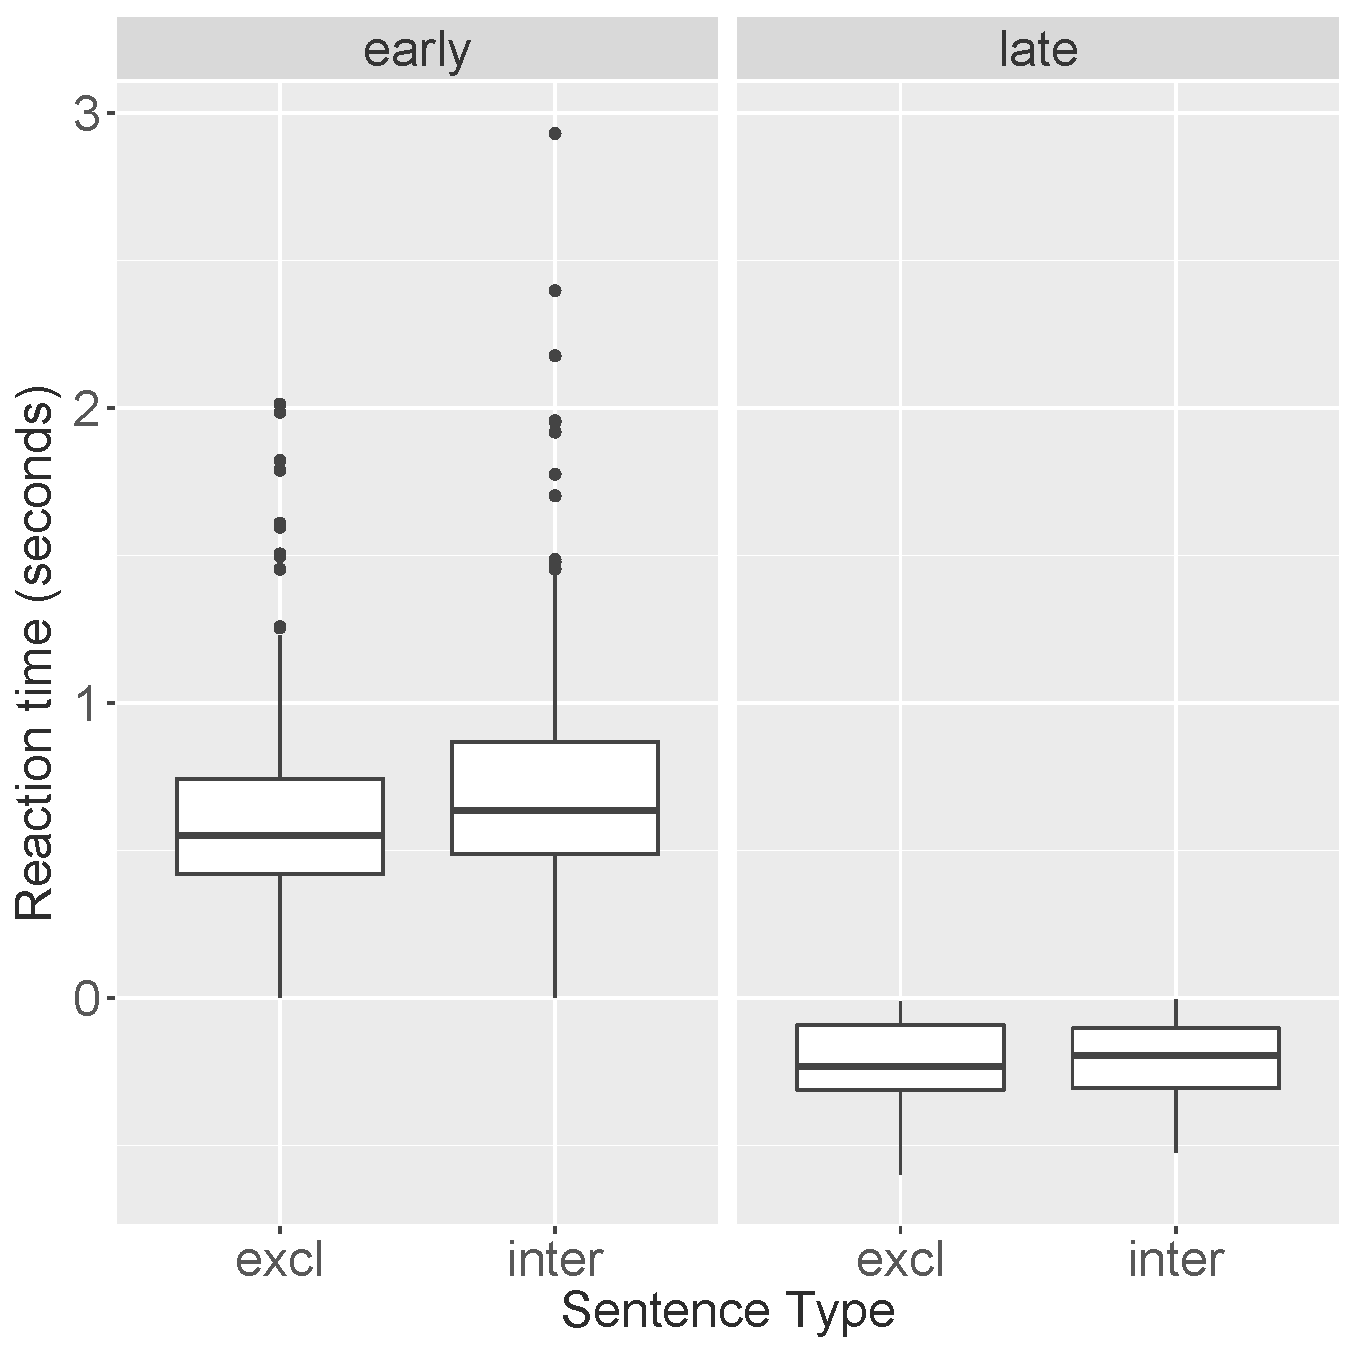
\includegraphics[width=0.7\textwidth]{figures/KEL-img3_big.png}
\caption{Reaction times (seconds) across \textit{sentence type} and \textit{response type}. The “0” value on the y-axis represents the end of the utterance, positive values represent RTs for responses given after the end of the utterance, and negative RTs correspond to responses given before the end of the utterance.}
\label{fig:kel:3}
\end{figure}


Given that the duration of the stimuli was different across the two sentence types (see \sectref{sec:kel:4}), we conducted another analysis that included the durations of the initial region (the \textit{wh-}phrase), the middle region (the verb phrase), and the final region (the subject phrase) as covariates. This analysis addressed the question of whether the difference in RT between \textit{wh-}exclamatives and \textit{wh-}interrogatives revealed by the above analyses was actually caused by \textit{sentence type} or whether it was an epiphenomenon resulting from the durational differences between the component regions of the \textit{wh-}exclamatives and the \textit{wh-}interrogatives. An LMM with \textit{sentence type}, \textit{response type}, and duration of \textit{initial region}, \textit{middle region}, and \textit{final region} as fixed factors and \textit{item} and \textit{participant} as random factors yields the following results. There is no significant difference across \textit{sentence type} ($\beta $  = 0.01, t = –0.77, p = .44) nor is there any interaction between \textit{sentence type} and \textit{response type} ($\beta $  = 0.1, t = –1.08, p = .28). Instead, \textit{response type} ($\beta $  = 1.2, t = 21.9, p < .001), \textit{initial region} ($\beta $  = –0.31, t = –4.15, p < .001), \textit{middle region} ($\beta $  = –0.23, t = –2.56, p < .02) and \textit{final region} ($\beta $  = –0.33, t = –5.51, p < .001) are significant. Hence, the results of this analysis show that the duration of each of the three regions of the sentence is a significant predictor of \textit{reaction times}, while the main factor of our experimental design, \textit{sentence type}, is not significant.



\section{Discussion and conclusions}
\label{sec:kel:6}
\largerpage

The identification task has shown that (Cosenza) Italian listeners are capable of distinguishing between \textit{wh-}exclamatives and \textit{wh-}interrogatives on the basis of prosody. The fact that listeners gave correct responses for both \textit{wh-}exclamatives and \textit{wh-}interrogatives in more than 90\% of trials indicates that there must be some prosodic marker that guides listeners’ judgments. Furthermore, this experiment was a preliminary attempt to find out whether prenuclear cues (like the \%H vs H* difference at the left edge of the IP) might be used for the purpose of pragmatic interpretation. The fact that our experiment elicited some early responses, roughly to the same degree in \textit{wh-}exclamatives (8.3\%) and \textit{wh-}interrogatives (9\%), is compatible with the hypothesis that listeners can employ prosodic information either in the nuclear region or in the prenuclear region to identify the sentence type. However, our results strongly support the hypothesis that the most relevant phonetic/phonological cues for sentence-type disambiguation are located at the end of the utterance, given that a) listeners gave their responses mostly (in more than 90\% of the cases) after the end of utterance; b) the early responses were provided on average about 200 ms before the end of the utterance and more than 2 seconds after the offset of the region containing the nuclear cues; and c) phonetic/phonological cues of the final region significantly affected the RTs. 

However, the fact that the duration of the initial and middle regions also significantly affected RT is strongly indicative that prosodic information in the prenuclear section might be exploited by listeners in identifying sentence type. If we take into account this last result, we might interpret the high rate of late responses as a result of listeners’ insecurity about their decision. Given that they were instructed to be both fast and accurate, listeners may have collected phonetic/phonological cues while listening to the utterance in order to increase the probability of a reliable response.\footnote{We thank a reviewer for pointing out this hypothesis to us.}

To conclude, our study has yielded important preliminary results concerning the identification and processing of \textit{wh-}exclamatives and \textit{wh-}interrogatives on the basis of prosody in Cosenza Italian. Listeners wait until the end of the utterance to respond in most but not all of the trials, thus suggesting that prosodic cues in the prenuclear contour are not strong enough by themselves to guide the pragmatic interpretation of the utterances in an unambiguous way. Furthermore, our study indicates that \textit{wh-}exclamatives are processed faster than \textit{wh-}interrogatives, but this effect disappears when the duration of different segmental regions of the utterance is taken into account.

\section{Benefits and challenges of the chosen method}
\label{sec:kel:7}

By combining an identification task with reaction time measurements, we measured not only accuracy in prosodic disambiguation (through the identification scores) but we also provided additional information about when exactly sentence-type identification takes place and whether one sentence type is more difficult to process than another (through reaction times).

We preferred this method to other offline tasks like the gating paradigm. In a gating paradigm, fragments of speech are presented to listeners in an order of increasing duration. Listeners usually have to identify these fragments and to rate their level of confidence. This method allows to obtain the location of the phonetic or phonological cue that is responsible for the correct identification \citep{Prieto.2012}. The gating paradigm has already been used in prosody research, particularly for investigating the contribution of the prenuclear contour to tune meaning (e.g. \citealt{Petrone2008,Petrone.2011,Sorianello2012,Prieto.2012}). One potential concern about this task is that stimuli consist in short pieces of artificially cut utterances, which might sound unnatural to listeners. Hence, the identification task might be more difficult to be accomplished. Furthermore, such a paradigm does not allow to track the continuous time course of utterance interpretation.

In the current study, we tried to overcome these concerns by using uncut stimuli, for which we tracked the course of utterance interpretation by means of reaction times. This seemed to us a simple technique that might be well suited for preliminary investigation of prosodic contrasts, such as the prosodic differences between \textit{wh-}exclamatives and \textit{wh-}interrogatives. However, our method did not clearly say whether the relevant phonological cues for sentence-type identification are included in the prenuclear region of the utterance or in the nuclear region. A potential problem with measuring RTs in an identification task in which listeners have to press a button is that there is a time delay between sentence-type identification and the response reaction (i.e., pressing the button). To address this issue, alternative methods for registering the response reaction could be implemented.

Online methods like eye-tracking or mouse tracking could be used (\citealt{Marslen-Wilson1992,Pynte1996,Tomlinson2011,Warren2014}). In particular, a methodological challenge concerning eye-tracking would be to develop a paradigm to investigate the time course of processing of intonational meaning (i.e., taking into account the meaning contribution of the prenuclear and nuclear sections) during visual search. For instance, in a study on American English, \citet{Heeren.2015} created a “targeted language game” by which an indirect association between different sentence types (questions and statements) and referents (objects on a visual display) is created. Analysis of gazes demonstrated that listeners can make an immediate use of the nuclear accents and boundary tones in processing questioning vs. asserting utterances. Their stimuli were however limited to less typical syntactic constructions of American English (elliptical utterances only containing the nucleus), so the contribution of the prenuclear section was unclear. In an eye-tracking experiment on French, \citet{petroneETAL2016} combined long utterances produced with different degrees of commitment (as signaled by prosody: yes/no questions vs. incredulity questions) with pictures showing the corresponding facial expressions. Results indicated that French listeners can make immediate use of prenuclear cues for processing speaker commitment and that the effect of nuclear and prenuclear cues may vary across different utterance types. This kind of results encourages us to use the visual world paradigm to assess the use of intonation during sentence modality processing.

With regard to stimuli selection, the current experiment is based on natural stimuli and does not allow us to distinguish which acoustic marker contributed to listeners’ relatively high performance on sentence-type disambiguation at the end of the utterance. Our speaker produced \textit{wh-}ex\-cla\-ma\-tives and \textit{wh-}in\-ter\-ro\-ga\-tives based on specific pragmatic contexts, but she was not asked to produce a specific set of intonation contours. 

In future studies, we will investigate the influence of intonational cues (edge tones and pitch accents) by controlling for the tonal structure of the target sentences. When looking at intonational cues, durational differences could be controlled for by using resynthesized stimuli with similar segmental duration for \textit{wh-}exclamatives and \textit{wh-}interrogatives. Furthermore, a continuum of resynthesized stimuli could be used in order to determine whether the prosodic parameters under investigation are perceived in a categorical or gradient manner (see \citealt{Niebuhr2007}). 

\pagebreak

\section*{Appendix: Data Set}

% Please add the following required packages to your document preamble:
% \usepackage{multirow}


%\footnote{The numbers under M1 correspond to measurements of the duration from the beginning of the acoustic file to the beginning of the utterance.}

\begin{table}
\begin{tabularx}{\textwidth}{ll}
\lsptoprule
Vieni stasera? & `Will you come tonight?’                    \\
Mi fai un caffè? & `Would you prepare me a coffee?’          \\
Apriresti la finestra? & `Would you open the window?’        \\
Piove tanto? & `Does it rain a lot?’                          \\
Sei bella? & `Are you beatiful?’                             \\
Mi daresti il tuo numero? & `Would you tell me your number?’ \\
Perchè piangi? & `Why do you cry?’                           \\
Hai visto il mio ragazzo? & `Did you see my boyfriend?’     \\
Hai 25 anni? & `Are you 25 years old?’                       \\
Sei una stronza! & `You are stupid?’                         \\
C´è qualcuno al telefono! & `There is someone on the phone!’ \\
Forse hai ragione! & `Maybe you are right!’                  \\
Sei una persona speciale! & `You are a special person!’      \\
Vieni sta sera! & `Come tonight!’                            \\
Guarda 'sto video! & `Watch this video!’                     \\
Sei bellissima! & `You are beautiful!’          			\\            
\lspbottomrule
\end{tabularx}
\caption{Itemlist\_Fillers}
\label{tab:kel:2}
\end{table}

\begin{table}
\footnotesize
\resizebox{.9\columnwidth}{!}{
\begin{tabular}{lrrrr}
\lsptoprule
Target sentences & \multicolumn{4}{c}{Placement of dur. markers (sec)} \\\cmidrule(lr){2-5}
                                                               & M1     & M2            & M3            & M4            \\\midrule
Quanti romanzi ha scritto la tua amica                         & 1.052  &  1.733         & 2.252         & 3.127         \\
`How many novels did your friend write?’                       &        &                &               &               \\
Quanti libri ha pubblicato il tuo professore                   & 1.367  &  1.828         & 2.507         & 3.596         \\
`How many books did your professor publish?’                   &        &                &               &               \\
Quante sigarette ha fumato papa                                & 1.219  &  1.926         & 2.595         & 3.074         \\
`How many cigarettes did Dad smoke?’                           &        &                &               &               \\
Quanti paesi ha visto tua sorella                              & 1.141  &  1.651         & 2.138         & 2.847         \\
`How many countries did your sister see?’                      &        &                &               &               \\
Quante cose ha aggiustato tuo padre                            & 1.421  &  1.996         & 2.587         & 3.169         \\
`How many things did your father adjust?’                      &        &                &               &               \\
Quante birre ha bevuto la tua amica                            & 0.999  &  1.490         & 2.052         & 2.747         \\
`How many beers did your friend drink?’                        &        &                &               &               \\
Quanti chili ha perso tuo nipote                               & 0.895  &  1.351         & 1.870         & 2.613         \\
`How many kilos did your nephew loose?’                        &        &                &               &               \\
Quanti corsi ha seguito tua sorella                            & 1.094  &  1.577         & 2.222         & 3.069         \\
`How many lectures did your sister take?’                      &        &                &               &               \\
Quanta torta ha mangiato tua sorella                           & 1.090  &  1.618         & 2.222         & 3.059         \\
`How much cake did your sister eat?’                            &        &                &               &               \\
Quanti libri ha comprato tuo padre                             & 0.809  &  1.285         & 1.965         & 2.710         \\
`How many books did your father buy?’                           &        &                &               &               \\
Quanti soldi ti ha dato tuo padre                              & 1.186  &  1.778         & 2.280         & 2.935         \\
`How much money did your father give you?’                      &        &                &               &               \\
Quanti vestiti ha disegnato il tuo amico                       & 1.049  &  1.684         & 2.285         & 3.100         \\
`How many clothes did your friend design?’                      &        &                &               &               \\
Quanti pesci ha pescato tuo fratello                           & 1.130  &  1.626         & 2.249         & 3.113         \\
`How much fish did your brother catch?’                         &        &                &               &               \\
Quanti cd ha inciso tuo zio                                    & 1.124  &  1.739         & 2.256         & 3.013         \\
`How many discs did your uncle record?’                         &        &                &               &               \\
Quante arance ha raccolto tuo nonno                            & 1.335  &  1.860         & 2.494         & 3.169         \\
`How many oranges did your grandfather                         &        &                &               &               \\
collect?’                                                      &        &                &               &               \\
Quanti quadri ha dipinto tua zia                               & 1.197  &  1.688         & 2.325         & 3.055         \\
`How many paintings did your aunt paint?’                      &        &                &               &               \\
Quanti dolci ha preparato tua madre                            & 1.230  &  1.751         & 2.402         & 3.149         \\
`How many sweets did your mother prepare?’                     &        &                &               &               \\
Quanti fiori ha piantato tua nonna                             & 1.413  &  1.887         & 2.492         & 3.255         \\
`How many flowers did your grandmother plant?’                 &        &                &               &               \\
Quante farfalle ha catturato tuo fratello                      & 0.624  &  1.266         & 1.926         & 2.759         \\
`How many butterflies did your brother capture?’               &        &                &               &               \\
Quante scarpe ha comprato tua zia                              & 1.219  &  1.780         & 2.476         & 3.063         \\
`How many shoes did your aunt buy?’                            &        &                &               &               \\
\lspbottomrule
\end{tabular}
}
\caption{Duration markers according to target sentences (Interrogatives)}
\label{tab:kel:3}
\end{table}



\begin{table}
\footnotesize
\resizebox{\columnwidth}{!}{
\begin{tabular}{lrrrr}
\lsptoprule
Target sentences & \multicolumn{4}{c}{Placement of dur. markers (sec)} \\\midrule                                                               
Quanti romanzi ha scritto la tua amica                         & 1.286  &  1.985         & 2.575         & 3.438         \\
`How many novels your friend wrote!’                           &        &                &               &               \\
Quanti libri ha pubblicato il tuo professore                   & 1.087  &  1.655         & 2.356         & 3.570         \\
`How many books your professor published!’                     &        &                &               &               \\
Quante sigarette ha fumato papa                                & 1.098  &  1.960         & 2.737         & 3.348         \\
`How many cigarettes Dad smoked!’                              &        &                &               &               \\
Quanti paesi ha visto tua sorella                              & 1.076  &  1.600         & 2.062         & 2.970         \\
`How many countries your sister saw!’                          &        &                &               &               \\
Quante cose ha aggiustato tuo padre                            & 1.030  &  1.553         & 2.235         & 3.044         \\
`How many things your father adjusted!’                        &        &                &               &               \\
Quante birre ha bevuto la tua amica                            & 1.097  &  1.619         & 2.174         & 3.180         \\
`How many beers your friend drunk!’                             &        &                &               &               \\
Quanti chili ha perso tuo nipote                               & 0.891  &  1.307         & 1.800         & 2.673         \\
`How many kilos your nephew lost!’                             &        &                &               &               \\
Quanti corsi ha seguito tua sorella                            & 1.207  &  1.766         & 2.237         & 3.237         \\
`How many lectures your sister took!’                          &        &                &               &               \\
Quanta torta ha mangiato tua sorella                           & 1.068  &  1.645         & 2.158         & 3.032         \\
`How much cake your sister ate!’                               &        &                &               &               \\
Quanti libri ha comprato tuo padre                             & 0.686  &  1.420         & 2.068         & 3.147         \\
`How many books your father bought!’                           &        &                &               &               \\
Quanti soldi ti ha dato tuo padre                              & 1.037  &  1.803         & 2.265         & 3.062         \\
`How much money your father gave you!’                         &        &                &               &               \\
Quanti vestiti ha disegnato il tuo amico                       & 0.942  &  1.828         & 2.454         & 3.361         \\
`How many clothes your friend designed!’                       &        &                &               &               \\
Quanti pesci ha pescato tuo fratello                           & 2.031  &  2.638         & 3.213         & 4.245         \\
`How much fish your brother catch!’                            &        &                &               &               \\
Quanti cd ha inciso tuo zio                                    & 1.143  &  1.886         & 2.346         & 3.226         \\
`How many discs your uncle recorded!’                          &        &                &               &               \\
Quante arance ha raccolto tuo nonno                            & 1.750  &  2.301         & 2.884         & 3.789         \\
`How many oranges your grandfather collected!’                 &        &                &               &               \\
Quanti quadri ha dipinto tua zia                               & 1.711  &  2.214         & 2.828         & 3.753         \\
`How many paintings your aunt painted!’                        &        &                &               &               \\
Quanti dolci ha preparato tua madre                            & 1.482  &  2.028         & 2.671         & 3.680         \\
`How many sweets your mother prepared!’                        &        &                &               &               \\
Quanti fiori ha piantato tua nonna                             & 1.335  &  1.802         & 2.463         & 3.486         \\
`How many flowers your grandmother planted!’                    &        &                &               &               \\
Quante farfalle ha catturato tuo fratello                      & 0.803  &  1.457         & 2.129         & 3.141         \\
`How many butterflies your brother captured!’                  &        &                &               &               \\
Quante scarpe ha comprato tua zia                              & 1.054  &  1.670         & 2.316         & 3.240         \\
`How many shoes your aunt bought!’                             &        &                &               &     \\
\lspbottomrule
\end{tabular}
}
\caption{Duration markers according to target sentences (Exclamatives)}
\label{tab:kel:4}
\end{table}


\clearpage


{\sloppy
\printbibliography[heading=subbibliography,notkeyword=this]
}

\end{document}
